\documentclass[twoside]{book}

% Packages required by doxygen
\usepackage{fixltx2e}
\usepackage{calc}
\usepackage{doxygen}
\usepackage[export]{adjustbox} % also loads graphicx
\usepackage{graphicx}
\usepackage[utf8]{inputenc}
\usepackage{makeidx}
\usepackage{multicol}
\usepackage{multirow}
\PassOptionsToPackage{warn}{textcomp}
\usepackage{textcomp}
\usepackage[nointegrals]{wasysym}
\usepackage[table]{xcolor}

% NLS support packages
\usepackage[french]{babel}

% Font selection
\usepackage[T1]{fontenc}
\usepackage[scaled=.90]{helvet}
\usepackage{courier}
\usepackage{amssymb}
\usepackage{sectsty}
\renewcommand{\familydefault}{\sfdefault}
\allsectionsfont{%
  \fontseries{bc}\selectfont%
  \color{darkgray}%
}
\renewcommand{\DoxyLabelFont}{%
  \fontseries{bc}\selectfont%
  \color{darkgray}%
}
\newcommand{\+}{\discretionary{\mbox{\scriptsize$\hookleftarrow$}}{}{}}

% Page & text layout
\usepackage{geometry}
\geometry{%
  a4paper,%
  top=2.5cm,%
  bottom=2.5cm,%
  left=2.5cm,%
  right=2.5cm%
}
\tolerance=750
\hfuzz=15pt
\hbadness=750
\setlength{\emergencystretch}{15pt}
\setlength{\parindent}{0cm}
\setlength{\parskip}{3ex plus 2ex minus 2ex}
\makeatletter
\renewcommand{\paragraph}{%
  \@startsection{paragraph}{4}{0ex}{-1.0ex}{1.0ex}{%
    \normalfont\normalsize\bfseries\SS@parafont%
  }%
}
\renewcommand{\subparagraph}{%
  \@startsection{subparagraph}{5}{0ex}{-1.0ex}{1.0ex}{%
    \normalfont\normalsize\bfseries\SS@subparafont%
  }%
}
\makeatother

% Headers & footers
\usepackage{fancyhdr}
\pagestyle{fancyplain}
\fancyhead[LE]{\fancyplain{}{\bfseries\thepage}}
\fancyhead[CE]{\fancyplain{}{}}
\fancyhead[RE]{\fancyplain{}{\bfseries\leftmark}}
\fancyhead[LO]{\fancyplain{}{\bfseries\rightmark}}
\fancyhead[CO]{\fancyplain{}{}}
\fancyhead[RO]{\fancyplain{}{\bfseries\thepage}}
\fancyfoot[LE]{\fancyplain{}{}}
\fancyfoot[CE]{\fancyplain{}{}}
\fancyfoot[RE]{\fancyplain{}{\bfseries\scriptsize Généré par Doxygen }}
\fancyfoot[LO]{\fancyplain{}{\bfseries\scriptsize Généré par Doxygen }}
\fancyfoot[CO]{\fancyplain{}{}}
\fancyfoot[RO]{\fancyplain{}{}}
\renewcommand{\footrulewidth}{0.4pt}
\renewcommand{\chaptermark}[1]{%
  \markboth{#1}{}%
}
\renewcommand{\sectionmark}[1]{%
  \markright{\thesection\ #1}%
}

% Indices & bibliography
\usepackage{natbib}
\usepackage[titles]{tocloft}
\setcounter{tocdepth}{3}
\setcounter{secnumdepth}{5}
\makeindex

% Hyperlinks (required, but should be loaded last)
\usepackage{ifpdf}
\ifpdf
  \usepackage[pdftex,pagebackref=true]{hyperref}
\else
  \usepackage[ps2pdf,pagebackref=true]{hyperref}
\fi
\hypersetup{%
  colorlinks=true,%
  linkcolor=blue,%
  citecolor=blue,%
  unicode%
}

% Custom commands
\newcommand{\clearemptydoublepage}{%
  \newpage{\pagestyle{empty}\cleardoublepage}%
}

\usepackage{caption}
\captionsetup{labelsep=space,justification=centering,font={bf},singlelinecheck=off,skip=4pt,position=top}

%===== C O N T E N T S =====

\begin{document}

% Titlepage & ToC
\hypersetup{pageanchor=false,
             bookmarksnumbered=true,
             pdfencoding=unicode
            }
\pagenumbering{roman}
\begin{titlepage}
\vspace*{7cm}
\begin{center}%
{\Large Projet Huffman \\[1ex]\large 0.\+1 }\\
\vspace*{1cm}
{\large Généré par Doxygen 1.8.11}\\
\end{center}
\end{titlepage}
\clearemptydoublepage
\tableofcontents
\clearemptydoublepage
\pagenumbering{arabic}
\hypersetup{pageanchor=true}

%--- Begin generated contents ---
\chapter{consignes}
\label{md_A_FAIRE}
\hypertarget{md_A_FAIRE}{}

\begin{DoxyItemize}
\item corrigé docs
\item netoyer l\textquotesingle{}archive
\item les listings (fichiers sources) documentés (doxygen) P\+A\+P\+I\+ER
\begin{DoxyItemize}
\item doxygen
\item cd/latex
\item make
\end{DoxyItemize}
\item Archive nommée par les noms du groupe
\item Envoyer à \href{mailto:meynard@lirmm.fr}{\tt meynard@lirmm.\+fr} et \href{mailto:pompidor@lirmm.fr}{\tt pompidor@lirmm.\+fr}
\end{DoxyItemize}






\begin{DoxyItemize}
\item Quel est le nombre maximum de caractères (char) différents ?
\begin{DoxyItemize}
\item Le nombre maximum de caractères est 256.
\end{DoxyItemize}
\item Comment représenter l’arbre de Huffman ? Si l’arbre est implémenté avec des tableaux (fg, fd, parent), quels sont les indices des feuilles ? Quelle est la taille maximale de l’arbre (nombre de noeuds) ?
\begin{DoxyItemize}
\item L\textquotesingle{}arbre de huffman est représenté par une structure possédant les varriables {\ttfamily pere},{\ttfamily fg}, {\ttfamily fd} et {\ttfamily frequences}.
\item Si l’arbre est implémenté avec des tableaux (fg, fd, parent), les indices des feuilles corresponde au code du carractère.
\item L\textquotesingle{}arbre peut avoir au maximum 256 Noeuds.
\end{DoxyItemize}
\item Comment les caractères présents sont-\/ils codés dans l’arbre ?
\begin{DoxyItemize}
\item il sont codé par leurs code A\+S\+Cii.
\end{DoxyItemize}
\item Le préfixe du fichier compressé doit-\/il nécessairement contenir l’arbre ou les codes des caractères ou bien les deux (critère d’efficacité) ?
\begin{DoxyItemize}
\item Le préfixe du fichier compressé doit contenir soit l\textquotesingle{}arbre soit les codes des caractères.
\item Stocker l\textquotesingle{}arbre est plus efficace en terme de taille de stokage ainsi qu\textquotesingle{}en efficacité lors de la décomprétion.
\end{DoxyItemize}
\item Quelle est la taille minimale de ce préfixe (expliquer chaque champ et sa longueur) ?
\begin{DoxyItemize}
\item Le préfixe est composé de 3 octet magiques (Pas obligatoire) permétant d\textquotesingle{}identifié pouvant être décompréssé. 1 octet représentant le nombre de bits utile du dernier octet puis l\textquotesingle{}arbre.
\end{DoxyItemize}
\item Si le dernier caractère écrit ne finit pas sur une frontière d’octet, comment le compléter ? Comment ne pas prendre les bits de complétion pour des bits de données ?
\begin{DoxyItemize}
\item on le complete avc des 0 inutile.
\item Lors de la décomprétion on vérifie si on est sur le dernier octet, si c\textquotesingle{}est le cas on ne traite que les bits utile. le nombre de bits utile a été récupéré dans l\textquotesingle{}entête.
\end{DoxyItemize}
\item Le décompresseur doit-\/il reconstituer l’arbre ? Comment ?
\begin{DoxyItemize}
\item oui, a partir de l\textquotesingle{}entête. Dans notre cas l\textquotesingle{}arbre est reconstruit dans un tableau de {\ttfamily Noeuds}. 
\end{DoxyItemize}
\end{DoxyItemize}
\chapter{R\+E\+A\+D\+ME}
\label{md_README}
\hypertarget{md_README}{}
Dans le cadre de l\textquotesingle{}UE Systèmes d\textquotesingle{}exploitation (H\+L\+I\+N303) nous avons réalisé un compresseur sans perte utilisant l\textquotesingle{}algorithme de Huffman.

\subsection*{État d\textquotesingle{}avancement du projet}

Nous avons terminé le compresseur ainsi que le décompresseur. Nous n\textquotesingle{}avons pas pu réaliser l’archiveur Python demandé dans le sujet par manque de temps.

Si nous avions eu plus de temps, nous aurions stocké l\textquotesingle{}arbre bit par bit au lieu de octet par octet.

\subsection*{Cas testés}

Nous avons testé avec succès notre compresseur sur les fichiers suivants \+:
\begin{DoxyItemize}
\item un fichier vide
\item un fichier ne comportant qu\textquotesingle{}un seul type de caractère
\item un fichier comportant tous les caractères
\item fichiers textes sans particularités
\item autres types de fichiers \+: images, vidéos, ...
\end{DoxyItemize}

\subsection*{Bug résiduels}

Tous les bugs rencontrés ont été corrigés. Après de nombreux tests, nous n\textquotesingle{}en avons pas trouvé de nouveaux. 
\chapter{Index des structures de données}
\section{Structures de données}
Liste des structures de données avec une brève description \+:\begin{DoxyCompactList}
\item\contentsline{section}{\hyperlink{structnoeud}{noeud} \\*Noeud d\textquotesingle{}un arbre binaire }{\pageref{structnoeud}}{}
\end{DoxyCompactList}

\chapter{Index des fichiers}
\section{Liste des fichiers}
Liste de tous les fichiers documentés avec une brève description \+:\begin{DoxyCompactList}
\item\contentsline{section}{compresseur/include/\hyperlink{codeBin_8h}{code\+Bin.\+h} \\*Déclaration de la fonction qui va générer les codes binaires }{\pageref{codeBin_8h}}{}
\item\contentsline{section}{compresseur/include/\hyperlink{constrcArbre_8h}{constrc\+Arbre.\+h} \\*Déclaration de la fonction qui va construire l\textquotesingle{}arbre }{\pageref{constrcArbre_8h}}{}
\item\contentsline{section}{compresseur/include/\hyperlink{compresseur_2include_2defNoeud_8h}{def\+Noeud.\+h} \\*Définit la structure Noeud }{\pageref{compresseur_2include_2defNoeud_8h}}{}
\item\contentsline{section}{compresseur/include/\hyperlink{frequences_8h}{frequences.\+h} \\*Définit la fonction de génération des fréquences }{\pageref{frequences_8h}}{}
\item\contentsline{section}{compresseur/include/\hyperlink{generation_8h}{generation.\+h} \\*Déclaration de la fonction de génération du fichier compressé }{\pageref{generation_8h}}{}
\item\contentsline{section}{decompresseur/include/\hyperlink{decompresseur_8h}{decompresseur.\+h} }{\pageref{decompresseur_8h}}{}
\item\contentsline{section}{decompresseur/include/{\bfseries def\+Noeud.\+h} }{\pageref{decompresseur_2include_2defNoeud_8h}}{}
\end{DoxyCompactList}

\chapter{Documentation des structures de données}
\hypertarget{structnoeud}{}\section{Référence de la structure noeud}
\label{structnoeud}\index{noeud@{noeud}}


Noeud d\textquotesingle{}un arbre binaire.  




{\ttfamily \#include $<$def\+Noeud.\+h$>$}

\subsection*{Champs de données}
\begin{DoxyCompactItemize}
\item 
unsigned int \hyperlink{structnoeud_aa5b03ff1fc332c2390f0324398c0ee1d}{pere}
\item 
unsigned int \hyperlink{structnoeud_ae14c26edcd37240fc9f8e3769d55d3e5}{fg}
\item 
unsigned int \hyperlink{structnoeud_a72ced58e381fdf4144d295884dcd7168}{fd}
\item 
double \hyperlink{structnoeud_a27b27306f715b45b8f8e47bb35ad3859}{frequences}
\end{DoxyCompactItemize}


\subsection{Description détaillée}
Noeud d\textquotesingle{}un arbre binaire. 

Noeud est une petite structure comportant les indices de son noeud père et de ses noeuds fils. Lui est également associé la fréquence d\textquotesingle{}apparation dans un fichier du caractère associé à ce noeud. 

\subsection{Documentation des champs}
\index{noeud@{noeud}!fd@{fd}}
\index{fd@{fd}!noeud@{noeud}}
\subsubsection[{\texorpdfstring{fd}{fd}}]{\setlength{\rightskip}{0pt plus 5cm}unsigned int noeud\+::fd}\hypertarget{structnoeud_a72ced58e381fdf4144d295884dcd7168}{}\label{structnoeud_a72ced58e381fdf4144d295884dcd7168}
Indices du fils droit \index{noeud@{noeud}!fg@{fg}}
\index{fg@{fg}!noeud@{noeud}}
\subsubsection[{\texorpdfstring{fg}{fg}}]{\setlength{\rightskip}{0pt plus 5cm}unsigned int noeud\+::fg}\hypertarget{structnoeud_ae14c26edcd37240fc9f8e3769d55d3e5}{}\label{structnoeud_ae14c26edcd37240fc9f8e3769d55d3e5}
Indices du fils gauche \index{noeud@{noeud}!frequences@{frequences}}
\index{frequences@{frequences}!noeud@{noeud}}
\subsubsection[{\texorpdfstring{frequences}{frequences}}]{\setlength{\rightskip}{0pt plus 5cm}double noeud\+::frequences}\hypertarget{structnoeud_a27b27306f715b45b8f8e47bb35ad3859}{}\label{structnoeud_a27b27306f715b45b8f8e47bb35ad3859}
Fréquence d\textquotesingle{}apparation du caractère lié au noeud \index{noeud@{noeud}!pere@{pere}}
\index{pere@{pere}!noeud@{noeud}}
\subsubsection[{\texorpdfstring{pere}{pere}}]{\setlength{\rightskip}{0pt plus 5cm}unsigned int noeud\+::pere}\hypertarget{structnoeud_aa5b03ff1fc332c2390f0324398c0ee1d}{}\label{structnoeud_aa5b03ff1fc332c2390f0324398c0ee1d}
Indices du noeud père 

La documentation de cette structure a été générée à partir du fichier suivant \+:\begin{DoxyCompactItemize}
\item 
compresseur/include/\hyperlink{compresseur_2include_2defNoeud_8h}{def\+Noeud.\+h}\end{DoxyCompactItemize}

\chapter{Documentation des fichiers}
\hypertarget{codeBin_8h}{}\section{Référence du fichier compresseur/include/code\+Bin.h}
\label{codeBin_8h}\index{compresseur/include/code\+Bin.\+h@{compresseur/include/code\+Bin.\+h}}


Déclaration de la fonction qui va générer les codes binaires.  


{\ttfamily \#include \char`\"{}def\+Noeud.\+h\char`\"{}}\\*
Graphe des dépendances par inclusion de code\+Bin.\+h\+:\nopagebreak
\begin{figure}[H]
\begin{center}
\leavevmode
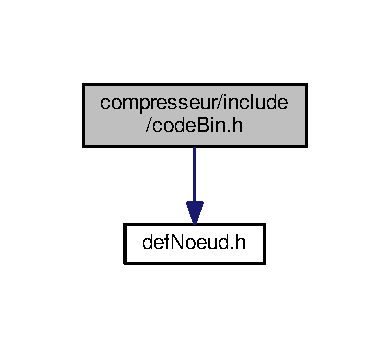
\includegraphics[width=187pt]{codeBin_8h__incl}
\end{center}
\end{figure}
\subsection*{Fonctions}
\begin{DoxyCompactItemize}
\item 
char $\ast$$\ast$ \hyperlink{codeBin_8h_a621215604ceaeeba93074a0054b61afa}{Code\+Bin} (\hyperlink{compresseur_2include_2defNoeud_8h_aff1a0e48483c61f8f52fee44eccc3f42}{Noeud} $\ast$arbre, int racine)
\begin{DoxyCompactList}\small\item\em Génère les codes binaires. \end{DoxyCompactList}\end{DoxyCompactItemize}


\subsection{Description détaillée}
Déclaration de la fonction qui va générer les codes binaires. 



\subsection{Documentation des fonctions}
\index{code\+Bin.\+h@{code\+Bin.\+h}!Code\+Bin@{Code\+Bin}}
\index{Code\+Bin@{Code\+Bin}!code\+Bin.\+h@{code\+Bin.\+h}}
\subsubsection[{\texorpdfstring{Code\+Bin(\+Noeud $\ast$arbre, int racine)}{CodeBin(Noeud *arbre, int racine)}}]{\setlength{\rightskip}{0pt plus 5cm}char$\ast$$\ast$ Code\+Bin (
\begin{DoxyParamCaption}
\item[{{\bf Noeud} $\ast$}]{arbre, }
\item[{int}]{racine}
\end{DoxyParamCaption}
)}\hypertarget{codeBin_8h_a621215604ceaeeba93074a0054b61afa}{}\label{codeBin_8h_a621215604ceaeeba93074a0054b61afa}


Génère les codes binaires. 

Ces codes binaires sont associés à chaque caractère présent dans le fichier d\textquotesingle{}origine.


\begin{DoxyParams}{Paramètres}
{\em arbre} & Arbre \\
\hline
{\em racine} & Indice de la racine de l\textquotesingle{}Arbre \\
\hline
\end{DoxyParams}
\begin{DoxyReturn}{Renvoie}
Index Tableau associant les codes binaires aux différents caractères 
\end{DoxyReturn}

\hypertarget{constrcArbre_8h}{}\section{Référence du fichier compresseur/include/constrc\+Arbre.h}
\label{constrcArbre_8h}\index{compresseur/include/constrc\+Arbre.\+h@{compresseur/include/constrc\+Arbre.\+h}}


Déclaration de la fonction qui va construire l\textquotesingle{}arbre.  


{\ttfamily \#include \char`\"{}def\+Noeud.\+h\char`\"{}}\\*
Graphe des dépendances par inclusion de constrc\+Arbre.\+h\+:
\nopagebreak
\begin{figure}[H]
\begin{center}
\leavevmode
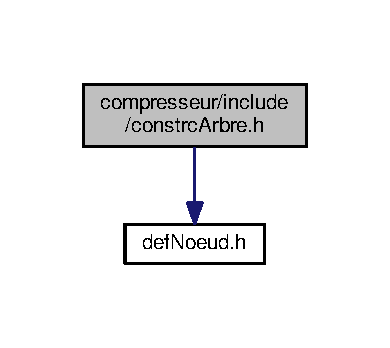
\includegraphics[width=187pt]{constrcArbre_8h__incl}
\end{center}
\end{figure}
\subsection*{Fonctions}
\begin{DoxyCompactItemize}
\item 
int \hyperlink{constrcArbre_8h_ae79a742ba5b273ece919e51cfd01e805}{Constrc\+Arbre} (double $\ast$tab\+\_\+frequence, \hyperlink{compresseur_2include_2defNoeud_8h_aff1a0e48483c61f8f52fee44eccc3f42}{Noeud} $\ast$arbre)
\begin{DoxyCompactList}\small\item\em Construction de l\textquotesingle{}arbre. \end{DoxyCompactList}\end{DoxyCompactItemize}


\subsection{Description détaillée}
Déclaration de la fonction qui va construire l\textquotesingle{}arbre. 



\subsection{Documentation des fonctions}
\index{constrc\+Arbre.\+h@{constrc\+Arbre.\+h}!Constrc\+Arbre@{Constrc\+Arbre}}
\index{Constrc\+Arbre@{Constrc\+Arbre}!constrc\+Arbre.\+h@{constrc\+Arbre.\+h}}
\subsubsection[{\texorpdfstring{Constrc\+Arbre(double $\ast$tab\+\_\+frequence, Noeud $\ast$arbre)}{ConstrcArbre(double *tab_frequence, Noeud *arbre)}}]{\setlength{\rightskip}{0pt plus 5cm}int Constrc\+Arbre (
\begin{DoxyParamCaption}
\item[{double $\ast$}]{tab\+\_\+frequence, }
\item[{{\bf Noeud} $\ast$}]{arbre}
\end{DoxyParamCaption}
)}\hypertarget{constrcArbre_8h_ae79a742ba5b273ece919e51cfd01e805}{}\label{constrcArbre_8h_ae79a742ba5b273ece919e51cfd01e805}


Construction de l\textquotesingle{}arbre. 


\begin{DoxyParams}{Paramètres}
{\em tab\+\_\+frequence} & Tableau des fréquences de répartition des caractères \\
\hline
{\em arbre} & Arbre préalablement initialisé \\
\hline
\end{DoxyParams}
\begin{DoxyReturn}{Renvoie}
Ind\+\_\+racine Indicide de la racine de l\textquotesingle{}arbre 
\end{DoxyReturn}

\hypertarget{compresseur_2include_2defNoeud_8h}{}\section{Référence du fichier compresseur/include/def\+Noeud.h}
\label{compresseur_2include_2defNoeud_8h}\index{compresseur/include/def\+Noeud.\+h@{compresseur/include/def\+Noeud.\+h}}


Définit la structure Noeud.  


Ce graphe montre quels fichiers incluent directement ou indirectement ce fichier \+:\nopagebreak
\begin{figure}[H]
\begin{center}
\leavevmode
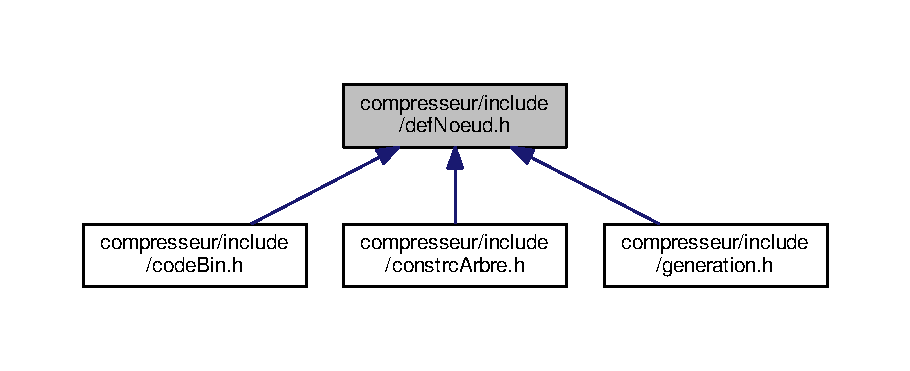
\includegraphics[width=350pt]{compresseur_2include_2defNoeud_8h__dep__incl}
\end{center}
\end{figure}
\subsection*{Structures de données}
\begin{DoxyCompactItemize}
\item 
struct \hyperlink{structnoeud}{noeud}
\begin{DoxyCompactList}\small\item\em Noeud d\textquotesingle{}un arbre binaire. \end{DoxyCompactList}\end{DoxyCompactItemize}
\subsection*{Définitions de type}
\begin{DoxyCompactItemize}
\item 
typedef struct \hyperlink{structnoeud}{noeud} \hyperlink{compresseur_2include_2defNoeud_8h_aff1a0e48483c61f8f52fee44eccc3f42}{Noeud}
\begin{DoxyCompactList}\small\item\em Noeud d\textquotesingle{}un arbre binaire. \end{DoxyCompactList}\end{DoxyCompactItemize}


\subsection{Description détaillée}
Définit la structure Noeud. 



\subsection{Documentation des définitions de type}
\index{compresseur/include/def\+Noeud.\+h@{compresseur/include/def\+Noeud.\+h}!Noeud@{Noeud}}
\index{Noeud@{Noeud}!compresseur/include/def\+Noeud.\+h@{compresseur/include/def\+Noeud.\+h}}
\subsubsection[{\texorpdfstring{Noeud}{Noeud}}]{\setlength{\rightskip}{0pt plus 5cm}typedef struct {\bf noeud} {\bf Noeud}}\hypertarget{compresseur_2include_2defNoeud_8h_aff1a0e48483c61f8f52fee44eccc3f42}{}\label{compresseur_2include_2defNoeud_8h_aff1a0e48483c61f8f52fee44eccc3f42}


Noeud d\textquotesingle{}un arbre binaire. 

Noeud est une petite structure comportant les indices de son noeud père et de ses noeuds fils. Lui est également associé la fréquence d\textquotesingle{}apparation dans un fichier du caractère associé à ce noeud. 
\hypertarget{decompresseur_2include_2defNoeud_8h}{}\section{Référence du fichier decompresseur/include/def\+Noeud.h}
\label{decompresseur_2include_2defNoeud_8h}\index{decompresseur/include/def\+Noeud.\+h@{decompresseur/include/def\+Noeud.\+h}}


Définit la structure Noeud.  


Ce graphe montre quels fichiers incluent directement ou indirectement ce fichier \+:
\nopagebreak
\begin{figure}[H]
\begin{center}
\leavevmode
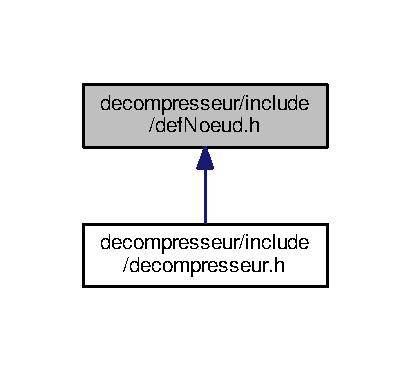
\includegraphics[width=197pt]{decompresseur_2include_2defNoeud_8h__dep__incl}
\end{center}
\end{figure}
\subsection*{Structures de données}
\begin{DoxyCompactItemize}
\item 
struct \hyperlink{structnoeud}{noeud}
\begin{DoxyCompactList}\small\item\em Noeud d\textquotesingle{}un arbre binaire. \end{DoxyCompactList}\end{DoxyCompactItemize}
\subsection*{Définitions de type}
\begin{DoxyCompactItemize}
\item 
typedef struct \hyperlink{structnoeud}{noeud} \hyperlink{decompresseur_2include_2defNoeud_8h_aff1a0e48483c61f8f52fee44eccc3f42}{Noeud}
\begin{DoxyCompactList}\small\item\em Noeud d\textquotesingle{}un arbre binaire. \end{DoxyCompactList}\end{DoxyCompactItemize}


\subsection{Description détaillée}
Définit la structure Noeud. 



\subsection{Documentation des définitions de type}
\index{decompresseur/include/def\+Noeud.\+h@{decompresseur/include/def\+Noeud.\+h}!Noeud@{Noeud}}
\index{Noeud@{Noeud}!decompresseur/include/def\+Noeud.\+h@{decompresseur/include/def\+Noeud.\+h}}
\subsubsection[{\texorpdfstring{Noeud}{Noeud}}]{\setlength{\rightskip}{0pt plus 5cm}typedef struct {\bf noeud} {\bf Noeud}}\hypertarget{decompresseur_2include_2defNoeud_8h_aff1a0e48483c61f8f52fee44eccc3f42}{}\label{decompresseur_2include_2defNoeud_8h_aff1a0e48483c61f8f52fee44eccc3f42}


Noeud d\textquotesingle{}un arbre binaire. 

Noeud est une petite structure comportant les indices de son noeud père et de ses noeuds fils. Lui est également associé la fréquence d\textquotesingle{}apparation dans un fichier du caractère associé à ce noeud 
\hypertarget{frequences_8h}{}\section{Référence du fichier compresseur/include/frequences.h}
\label{frequences_8h}\index{compresseur/include/frequences.\+h@{compresseur/include/frequences.\+h}}


Définit la fonction de génération des fréquences.  


{\ttfamily \#include $<$stdio.\+h$>$}\\*
Graphe des dépendances par inclusion de frequences.\+h\+:\nopagebreak
\begin{figure}[H]
\begin{center}
\leavevmode
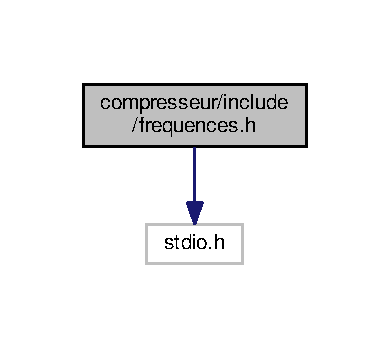
\includegraphics[width=187pt]{frequences_8h__incl}
\end{center}
\end{figure}
\subsection*{Fonctions}
\begin{DoxyCompactItemize}
\item 
double $\ast$ \hyperlink{frequences_8h_a553c3efaccc63f838769a8829eba15ed}{Calcul\+Frequences\+Caractere} (F\+I\+LE $\ast$fichier)
\begin{DoxyCompactList}\small\item\em Fonction de calcul de la répartition des fréquences dans un fichier. \end{DoxyCompactList}\end{DoxyCompactItemize}


\subsection{Description détaillée}
Définit la fonction de génération des fréquences. 



\subsection{Documentation des fonctions}
\index{frequences.\+h@{frequences.\+h}!Calcul\+Frequences\+Caractere@{Calcul\+Frequences\+Caractere}}
\index{Calcul\+Frequences\+Caractere@{Calcul\+Frequences\+Caractere}!frequences.\+h@{frequences.\+h}}
\subsubsection[{\texorpdfstring{Calcul\+Frequences\+Caractere(\+F\+I\+L\+E $\ast$fichier)}{CalculFrequencesCaractere(FILE *fichier)}}]{\setlength{\rightskip}{0pt plus 5cm}double$\ast$ Calcul\+Frequences\+Caractere (
\begin{DoxyParamCaption}
\item[{F\+I\+LE $\ast$}]{fichier}
\end{DoxyParamCaption}
)}\hypertarget{frequences_8h_a553c3efaccc63f838769a8829eba15ed}{}\label{frequences_8h_a553c3efaccc63f838769a8829eba15ed}


Fonction de calcul de la répartition des fréquences dans un fichier. 


\begin{DoxyParams}{Paramètres}
{\em fichier} & Fichier où les fréquences des caractères doivent être calculées \\
\hline
\end{DoxyParams}
\begin{DoxyReturn}{Renvoie}
tab\+\_\+frequence Un tableau contenant les fréquences des caractères contenus dans le fichier. L\textquotesingle{}indice d\textquotesingle{}une case correspond au code A\+S\+C\+II du caractère correspondant 
\end{DoxyReturn}

\hypertarget{generation_8h}{}\section{Référence du fichier compresseur/include/generation.h}
\label{generation_8h}\index{compresseur/include/generation.\+h@{compresseur/include/generation.\+h}}


Déclaration de la fonction de génération du fichier compressé  


{\ttfamily \#include $<$stdio.\+h$>$}\\*
{\ttfamily \#include \char`\"{}def\+Noeud.\+h\char`\"{}}\\*
Graphe des dépendances par inclusion de generation.\+h\+:
\nopagebreak
\begin{figure}[H]
\begin{center}
\leavevmode
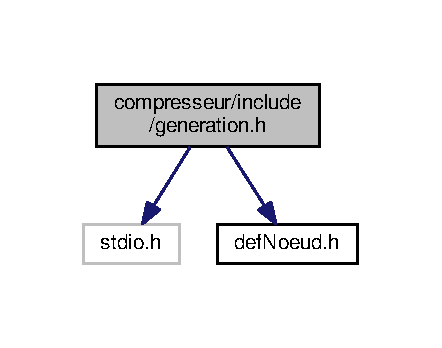
\includegraphics[width=212pt]{generation_8h__incl}
\end{center}
\end{figure}
\subsection*{Fonctions}
\begin{DoxyCompactItemize}
\item 
void \hyperlink{generation_8h_adc2a740eb2845a8ae19a32bb666f40cc}{Generation} (char $\ast$$\ast$index, F\+I\+LE $\ast$entre, F\+I\+LE $\ast$sortie, int racine, \hyperlink{compresseur_2include_2defNoeud_8h_aff1a0e48483c61f8f52fee44eccc3f42}{Noeud} $\ast$arbre)
\begin{DoxyCompactList}\small\item\em Ecrit dans le fichier \char`\"{}compressé\char`\"{} les codes binaires des caractères. \end{DoxyCompactList}\end{DoxyCompactItemize}


\subsection{Description détaillée}
Déclaration de la fonction de génération du fichier compressé 



\subsection{Documentation des fonctions}
\index{generation.\+h@{generation.\+h}!Generation@{Generation}}
\index{Generation@{Generation}!generation.\+h@{generation.\+h}}
\subsubsection[{\texorpdfstring{Generation(char $\ast$$\ast$index, F\+I\+L\+E $\ast$entre, F\+I\+L\+E $\ast$sortie, int racine, Noeud $\ast$arbre)}{Generation(char **index, FILE *entre, FILE *sortie, int racine, Noeud *arbre)}}]{\setlength{\rightskip}{0pt plus 5cm}void Generation (
\begin{DoxyParamCaption}
\item[{char $\ast$$\ast$}]{index, }
\item[{F\+I\+LE $\ast$}]{entre, }
\item[{F\+I\+LE $\ast$}]{sortie, }
\item[{int}]{racine, }
\item[{{\bf Noeud} $\ast$}]{arbre}
\end{DoxyParamCaption}
)}\hypertarget{generation_8h_adc2a740eb2845a8ae19a32bb666f40cc}{}\label{generation_8h_adc2a740eb2845a8ae19a32bb666f40cc}


Ecrit dans le fichier \char`\"{}compressé\char`\"{} les codes binaires des caractères. 


\begin{DoxyParams}{Paramètres}
{\em index} & Tableau de codes binaires associés aux différents caractères \\
\hline
{\em entre} & Fichier d\textquotesingle{}entrée \\
\hline
{\em sorti} & Fichier de sortie (fichier compressé) \\
\hline
{\em racine} & Indice de la racine de l\textquotesingle{}arbre \\
\hline
{\em arbre} & Arbre \\
\hline
\end{DoxyParams}

\hypertarget{decompresseur_8h}{}\section{Référence du fichier decompresseur/include/decompresseur.h}
\label{decompresseur_8h}\index{decompresseur/include/decompresseur.\+h@{decompresseur/include/decompresseur.\+h}}
{\ttfamily \#include $<$stdio.\+h$>$}\\*
{\ttfamily \#include \char`\"{}../include/def\+Noeud.\+h\char`\"{}}\\*
Graphe des dépendances par inclusion de decompresseur.\+h\+:
\nopagebreak
\begin{figure}[H]
\begin{center}
\leavevmode
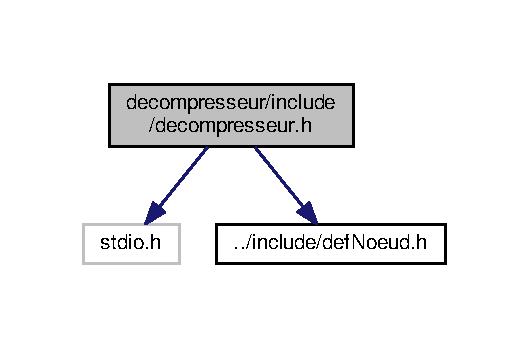
\includegraphics[width=254pt]{decompresseur_8h__incl}
\end{center}
\end{figure}
\subsection*{Macros}
\begin{DoxyCompactItemize}
\item 
\#define \hyperlink{decompresseur_8h_a7bd608453b83e74874a4983106a1d9cd}{E\+R\+R\+\_\+\+F\+O\+R\+M\+AT}~1\hypertarget{decompresseur_8h_a7bd608453b83e74874a4983106a1d9cd}{}\label{decompresseur_8h_a7bd608453b83e74874a4983106a1d9cd}

\begin{DoxyCompactList}\small\item\em Définit E\+R\+R\+\_\+\+F\+O\+R\+M\+AT = 1. \end{DoxyCompactList}\end{DoxyCompactItemize}
\subsection*{Fonctions}
\begin{DoxyCompactItemize}
\item 
int \hyperlink{decompresseur_8h_af0fd45634711c97682ab76904e95753e}{Decompression} (F\+I\+LE $\ast$Entree, F\+I\+LE $\ast$Sortie)
\begin{DoxyCompactList}\small\item\em Fonction permettant de décompresser un fichier. \end{DoxyCompactList}\end{DoxyCompactItemize}


\subsection{Description détaillée}
Déclaration de la fonction de décompression 

\subsection{Documentation des fonctions}
\index{decompresseur.\+h@{decompresseur.\+h}!Decompression@{Decompression}}
\index{Decompression@{Decompression}!decompresseur.\+h@{decompresseur.\+h}}
\subsubsection[{\texorpdfstring{Decompression(\+F\+I\+L\+E $\ast$\+Entree, F\+I\+L\+E $\ast$\+Sortie)}{Decompression(FILE *Entree, FILE *Sortie)}}]{\setlength{\rightskip}{0pt plus 5cm}int Decompression (
\begin{DoxyParamCaption}
\item[{F\+I\+LE $\ast$}]{Entree, }
\item[{F\+I\+LE $\ast$}]{Sortie}
\end{DoxyParamCaption}
)}\hypertarget{decompresseur_8h_af0fd45634711c97682ab76904e95753e}{}\label{decompresseur_8h_af0fd45634711c97682ab76904e95753e}


Fonction permettant de décompresser un fichier. 


\begin{DoxyParams}{Paramètres}
{\em Entree} & Fichier compressé d\textquotesingle{}entrée \\
\hline
{\em Sortie} & Fichier de sortie décompressé \\
\hline
\end{DoxyParams}
\begin{DoxyReturn}{Renvoie}
Retourne E\+R\+R\+\_\+\+F\+O\+R\+M\+AT si ce n\textquotesingle{}est pas un fichier qui peut être décompressé, retourne 0 sinon 
\end{DoxyReturn}

%--- End generated contents ---

% Index
\backmatter
\newpage
\phantomsection
\clearemptydoublepage
\addcontentsline{toc}{chapter}{Index}
\printindex

\end{document}
